\documentclass{article}
\usepackage[utf8]{inputenc}
\usepackage{multicol}
\usepackage{listings}
\usepackage{verbatim}
\usepackage{color}
\usepackage{geometry}

\usepackage{float}
\usepackage{amsmath}
\usepackage{hyperref}
\setlength{\belowcaptionskip}{-10pt}
\setlength{\abovecaptionskip}{-30pt}
\floatstyle{boxed} 
\restylefloat{figure}
\usepackage{graphicx}
\definecolor{codegreen}{rgb}{0,0.6,0}
\definecolor{codegray}{rgb}{0.5,0.5,0.5}
\definecolor{codepurple}{rgb}{0.58,0,0.82}
\definecolor{backcolour}{rgb}{0.95,0.95,0.92}

\lstdefinestyle{mystyle}{
	backgroundcolor=\color{backcolour},   
	commentstyle=\color{codegreen},
	keywordstyle=\color{blue},
	numberstyle=\tiny\color{codegray},
	stringstyle=\color{codepurple},
	basicstyle=\footnotesize,
	breakatwhitespace=false,         
	breaklines=true,                 
	captionpos=b,                    
	keepspaces=true,                 
	numbers=left,                    
	numbersep=5pt,                  
	showspaces=false,                
	showstringspaces=false,
	showtabs=false,                  
	tabsize=2
}

\lstset{style=mystyle}
\title{Image Processing\\
		Home work 01\\Different Types of Interpolation}
\author{\textbf{Student:}Aqeel Labash\\ \textbf{Teacher:} Gholamreza Anbarjafari}
\date{17 February 2016}
\geometry{
	a4paper,
	total={170mm,257mm},
	left=10mm,
	top=5mm,
}
\begin{document}
	\maketitle
\begin{multicols*}{2}
{\centering	\section{The Inverse Distance to a Power Method}}
As I understood it's the same of Shepard's method or Inverse Distance weighting\cite{1}. Simply the more distance between new point and the points around it the less effective it will be on the new point. It's given by following relation:
 \[
u(x)=\left\{
 \begin{array}{ll}
 \frac{\sum_{i=1}^{N}w_i(x_i) u_i}{\sum_{i=1}^{N}w_i(x_i)} , \textit{if } d(x,x_i) \neq 0 \\
 u_i,\hspace{15mm} \textit{if } d(x,x_i) =0
 \end{array}
 \right.
 \]
\[u_i= u(x_i) \text{ for } i=1,2...N \]
\[ w_i(x) = \frac{1}{d(x,x_i)^p} \]
From the previous formulas we notice that weight represent the influence this value on the new value.
 how much we are going to take from that neighbor.
{\centering	\section {The Kriging Method}}
The Kriging method also known as Gaussian processes is non-linear interpolation tool \cite{3}.Kriging method estimate point based on observed values (in our case pixels surrounding the new pixel) and it's defined by formula \cite{2}:
\[\hat{Z}_0 = \sum_{i=1}^{N} w_iZi \text{ where } \sum w_i=1 \]
The weights depend on the spatial covariance values.The advantages of Kirging \cite{4}
\begin{enumerate}
	\item Treat clusters as single point.
	\item Estimate of estimation error(Kriging variance.)
	\item "provide basis for stochastic simulation of possible realization of \(Z(u)\). \cite{4}
\end{enumerate}
{\centering	\section{The Minimum Curvature Method}}
\begin{flushleft}

This method is mainly used in earth science \cite{1}.It's "analgous to a thin,linearly elastic plate passing through each of the data values with a minimum amount of bending." \cite{5} It's also based on the modified biharmonic differential equation.
\end{flushleft}
{\centering	\section{The Modified Shepard's Method}	}
\begin{flushleft}

The modified Shepard's method differ from Shepard's method by using nearest neighbors in R-sphere\cite{3}.The weight is given by the following formula: 
\[w_k(x)=\left(\frac{max(0,R-d(x,x_k))}{Rd(x,x_k)}\right)^2\]
The previous formula allow to reduce the bull's-eye apperance of the generated contours.\cite{1}\cite{3}
\end{flushleft}
{\centering	\section{The Natural Neighbor Method}}
This method advantage is that it's provide smoother approximation and it use the following formula : \[G(x,y)=\sum_{i=1}^{n}w_i f(x_i,y_i)\] where \(w_i\) by "finding how much of each of the surrounding areas is "stolen" when inserting \((x,y)\) into the tessellation."\cite{6} where the values \((1,n)\) represent the surrounding area and \(f(x_i,y_i)\) represent specific area value.
\begin{figure}[H]
	\begin{center}
		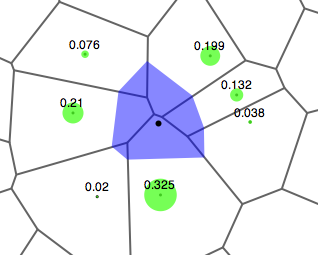
\includegraphics[scale=0.5]{Natural-neighbors-coefficients-example.png}
	\end{center}
\end{figure}
{\centering	\section{The Nearest Neighbor Method}}
\begin{flushleft}

In this method we assign the value of the nearest neighbor to the new pixel.This method useful when data evenly spaced.It could be used effectively if there isn't much points to be generated other wise it'll be problematic.\cite{1}
\end{flushleft}
{\centering	\section{The Polynomial Regression Method}}
\begin{flushleft}
This method try to find the patterns in the data and then predict the new point.it's general formula is :
\[y=a_0+a_1x+a_2x^2+a_3x^3+...+a_nx^n+\epsilon\]
after figuring out \(a_0,a_1,..,a_n\) we can predict the new points.
\end{flushleft}
{\centering	\section{The Radial Basis Function Interpolation Method}}
\begin{flushleft}
The value of this method depends only on the distance from the new point or pixel.\cite{7} There is many types for this method (Gaussian, multiquadric, inverse quadric, inverse multiquadric, polyharmonic spline,thin plate spline). It's approximation is given by the following formula: \[y(x) = \sum_{i=1}^{N}w_i\phi(||x-x_i||)\]
The multiquadrtic type is considered to be the best \cite{1} in producing smooth value.Which is considered by this formula :
\[\phi(r)=\sqrt{1+(\epsilon r)^2},r=||x-x_i||\]
The weights estimated by linear least squares due to the linearity of weights in the approximation function.\cite{7}
\end{flushleft}
{\centering	\section{The Triangulation Linear Interpolation Method}}
\begin{flushleft}
This method connect the points with triangles where no two share the same edge.This way any point would be identified by the three points of the triangle it belongs to. Best result from this method come out when the data are evenly distributed.\cite{1}
\end{flushleft}
{\centering	\section{The Moving Average Method}}
\begin{flushleft}
This method define a search ellipse with minimum number of data to use.To identify a point the ellipse will be centered at that point.The point value will be the average of all data points within ellipse.The ellipse should satisfy the minimum required number of data points other wise the value would be blanked.\cite{1}
\end{flushleft}
{\centering	\section{The Data Metrics Method}}
\begin{flushleft}
In this method we obtain the following information for each node : 
\begin{enumerate}
	\item number of point to interpolate.
	\item Standard deviation, variance, coefficient of variation,median absolute deviation.
	\item distance to the nearest point.
\end{enumerate}
So to get values for new point we use the nearest data metric to that point to calculate the new value.
\end{flushleft}
{\centering	\section{The Local Polynomial Method}}
\begin{flushleft}
This method use weighted least squared fit for data within the search ellipse to get the new value.It's given by the following formula for 2d pixel:
\[I(x,y)=\sum_{i,j=0}^{n}c_{ij}x^iy^i \] coefficient calculated by using the least square fit .\cite{8}\\ In this method the pixel is processed in blocks (3X3,4X4 etc..). This method can be used for image down-sampling, grey scale image compression,noise filtration.\cite{8}
\end{flushleft}
\begin{thebibliography}{9}
	
	\bibitem{1}
	\href{http://www.isprs.org/proceedings/xxxv/congress/comm2/papers/231.pdf}{Chin-Shung Yang* Szu-Pyng Kao* Fen-Bin Lee** Pen-Shang Hung** ,TWELVE DIFFERENT INTERPOLATION METHODS:A CASE STUDY OF SURFER 8.0}
	\bibitem{2}
	\href{http://www.imm.dtu.dk/~alan/krexample.pdf}{Kriging Example}
	\bibitem{3}
	\href{https://en.wikipedia.org/wiki/Interpolation}{Interpolation - Wikipedia}
	\bibitem{4}
	\href{http://people.ku.edu/~gbohling/cpe940/Kriging.pdf}{Krigin}
	\bibitem{5}
	\href{http://m.dressler.sweb.cz/AOSIM.pdf}{Mgr. Miroslav Dressler,Art of Surface Interpolation}
	\bibitem{6}
	Sibson, R. (1981). "A brief description of natural neighbor interpolation (Chapter 2)". In V. Barnett. Interpreting Multivariate Data. Chichester: John Wiley. pp. 21–36
	\bibitem{7}
	\href{https://en.wikipedia.org/wiki/Radial_basis_function#Approximation}{Radial basis function approximation}
	\bibitem{8}
	\href{http://www.hlevkin.com/articles/Local_polynomial_approximation.pdf}{Guennadi Levkine , In Vancouver, Canada, Image Local Polynomial Approximation (LPA) and it's Applications}
\end{thebibliography}
\end{multicols*}
\newpage
{\Huge{\centering\section*{PROGRAMMING PART}}}


\section*{Lanczos Function}
Lanczos kernel is given by the following formula:
\[L(x) = \Big\lbrace \begin{array}{ll}
sinc(x)sinc(\frac{x}{a})  , \text{ if } -a<x<a\\
0  \text{\hspace{23mm} other wise}
\end{array} \]
It's also can be written: 
\[
L(x) = \left\lbrace
\begin{array}{ll}
1 \hspace{23mm} \text{if } x=0\\
\frac{asin(\pi x)sin(\frac{\pi x}{a})}{\pi^2x^2} \hspace{3mm} \text{if } 0<|x|<a\\
0 \hspace{23mm} \text{other wise}
\end{array} \right.
\]

\section*{Methods Comparisons}
\subsection*{Before Start}
The Obelix image resolution is (2336,2724).
My picture resolution (429,592).
I decreased there resolution to (200,ratio). Here is the code for changing the resolution (considering aspect ratio) :
\begin{lstlisting}[language=Python]
obeleximg = cv2.imread("Obelix.jpg")
r = float(200)/float(obeleximg.shape[1])
dim = (200,int(obeleximg.shape[0]*r))
obeleximg = cv2.resize(obeleximg,dim)
cv2.imwrite("Obelexorignalgrayscal.png",obeleximg)

mypicture = cv2.imread("mypicture.JPG")
r = float(200)/float(mypicture.shape[1])
dim = (200,int(mypicture.shape[0]*r))
print dim
mypicture = cv2.resize(mypicture,dim)
cv2.imwrite("mupictureorignalgrayscal.png",mypicture)
\end{lstlisting}
\subsection*{Performance Comparisons}
After that I used python with opencv to double the images size for (Nearst,bilinear,bicubic) and used matlab for (lanczos ,spline).\\
The performance was as following Table measured in microseconds  : \\
\begin{tabular}{|c|c|c|c|c|c|}
\hline
Picture&lanczos4&Nearest&bilinear&bicubic&spline\\
\hline
Obelex&3951&375&508&849&100000\\
\hline
Me&1608&193&260&505&120000\\
\hline
\end{tabular}
And here is the code used to generate the pictures : 
\begin{lstlisting}[language=Python]
import cv2
from time import time

def InterpolateImage(img,way,filename):
	start = time()
	resized = cv2.resize(img,(img.shape[1]*2,img.shape[0]*2),interpolation=way)
	print filename+" : ", (time()-start)*1000000
	cv2.imwrite(filename+".png",resized)	 

InterpolateImage(obeleximg,cv2.INTER_NEAREST,'ObelexNearst')
InterpolateImage(obeleximg,cv2.INTER_LINEAR,'obelexBilinear')
InterpolateImage(obeleximg,cv2.INTER_CUBIC,'ObelexCubic')
InterpolateImage(obeleximg,cv2.INTER_LANCZOS4,'ObelexLanczos')

InterpolateImage(mypicture,cv2.INTER_NEAREST,'mypictureNearst')
InterpolateImage(mypicture,cv2.INTER_LINEAR,'mypictureBilinear')
InterpolateImage(mypicture,cv2.INTER_CUBIC,'mypictureCubic')
InterpolateImage(mypicture,cv2.INTER_LANCZOS4,'mypictureLanczos')
\end{lstlisting}
\newpage
\subsection*{Images Comparison}
\begin{figure}[H]
	\begin{center}
		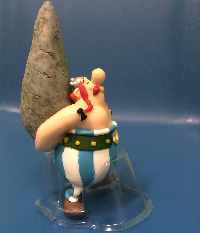
\includegraphics[scale=1]{Obelexorignalgrayscal.png}
		\end{center}
		\caption{Obelex original} 
		\end{figure}
This is the original image after resizing.
\begin{figure}[H]
	\begin{center}
		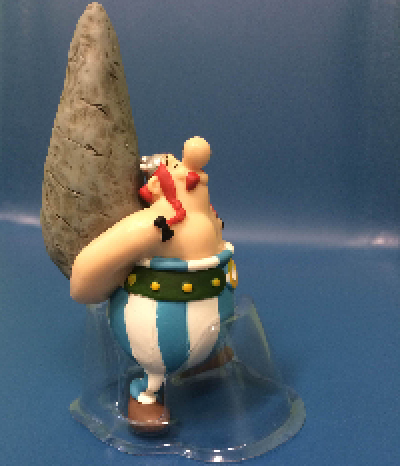
\includegraphics[scale=1]{ObelexNearst.png}
	\end{center}
	\caption{Obelex nearest  neighbor}
\end{figure}
In this image we can notice the squares every where.

\begin{figure}[H]
	\begin{center}
		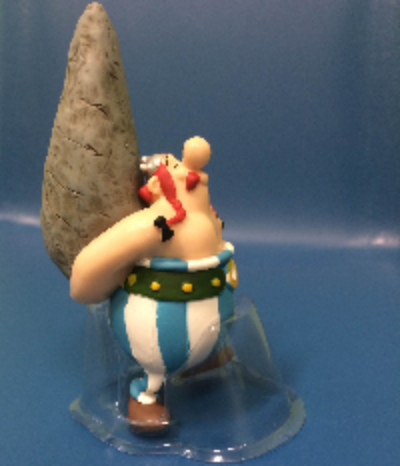
\includegraphics[scale=1]{obelexBilinear.png}
	\end{center}
	\caption{obelex Bilinear.png}
\end{figure}
In figure 3 we can notice that squares are less than figure 2 but still more blur 
\begin{figure}[H]
\begin{center}
		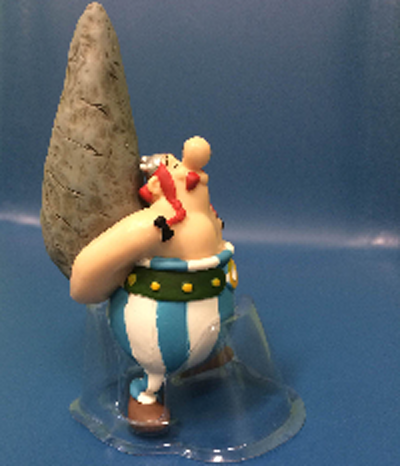
\includegraphics[scale=1]{ObelexCubic.png}
\end{center}
	\caption{Obelex Cubic}
\end{figure}
In figure 4 there still some squares but less blur than Bilinear (figure 3)
\begin{figure}[H]
\begin{center}
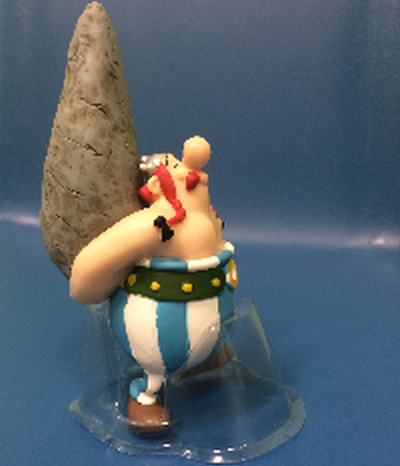
\includegraphics[scale=1]{oblexspline.png}
\end{center}
\caption{Obelix Spline}
\end{figure}
Here it has the same problems in figure 4 we still have squares but less than the previous techniques 
\begin{figure}[H]
\begin{center}
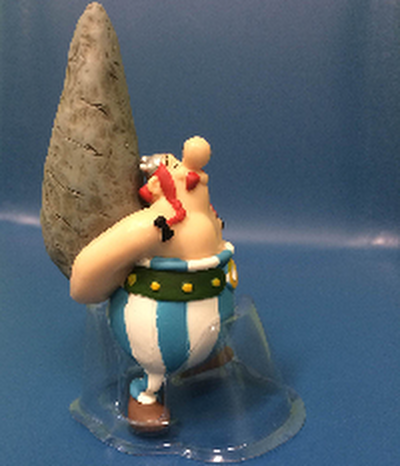
\includegraphics[scale=1]{ObelexLanczos.png}
\end{center}
\caption{Obelex Lanczos}
\end{figure}
Lanzos : so far the best one , least squares , least blur.\\
The implementation for Lanczos on Matlap is here ,main.m file :
\begin{lstlisting}[language = matlab]
obilixpicture = imread('Obelexorignalgrayscal.png');
mypicture=imread('mupictureorignalgrayscal.png');

obi_large = imresize(obilixpicture,2,{@lanczos4,4});
mypicturelarge=imresize(mypicture,2,{@lanczos4,4});

imwrite(mypicturelarge,'mypictureLanczos')
imwrite(obi_large,'ObelexLanczos')
\end{lstlisting}
and lanczos4.m
\begin{lstlisting}[language = matlab]
function f = lanczos4(x)
f = (sin(pi*x) .* sin(pi*x/4) + eps) ./ ((pi^2 * x.^2 / 4) + eps);
f = f .* (abs(x) <4);
end
\end{lstlisting}

\textbf{Note:} I used python code to generate the pictures, because I use linux and there was a problem executing the previous matlab code.
\begin{figure}[H]
	\begin{center}
		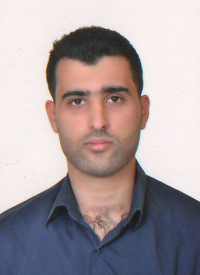
\includegraphics[scale=1]{mupictureorignalgrayscal.png}
	\end{center}
	\caption{My Picture original} 
\end{figure}
My picture after resizing.
\begin{figure}[H]
	\begin{center}
		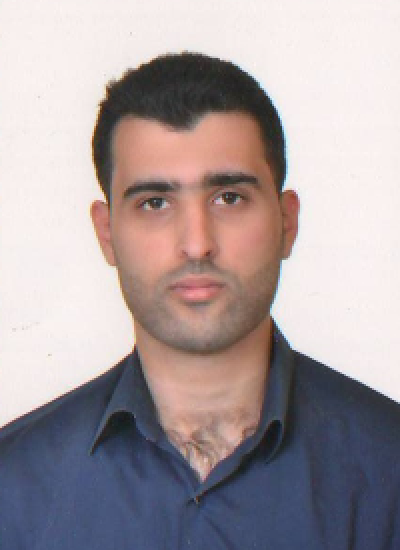
\includegraphics[scale=1]{mypictureNearst.png}
	\end{center}
	\caption{My Picture nearest  neighbor} 
\end{figure}
We notice squares everywhere here as well.
\begin{figure}[H]
	\begin{center}
		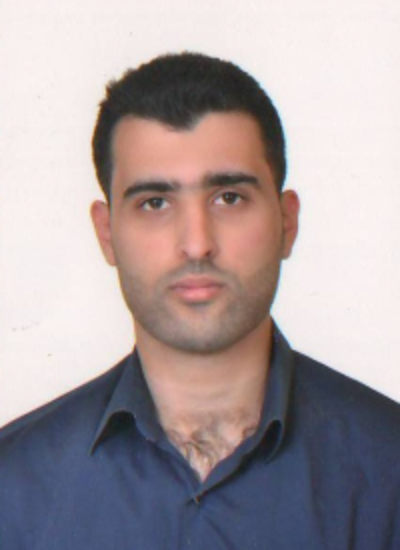
\includegraphics[scale=1]{mypictureBilinear.png}
	\end{center}
	\caption{My Picture Bilinear} 
\end{figure}
For Bilinear here actually some how I feel there is almost no squares but it is blur.
\begin{figure}[H]
	\begin{center}
		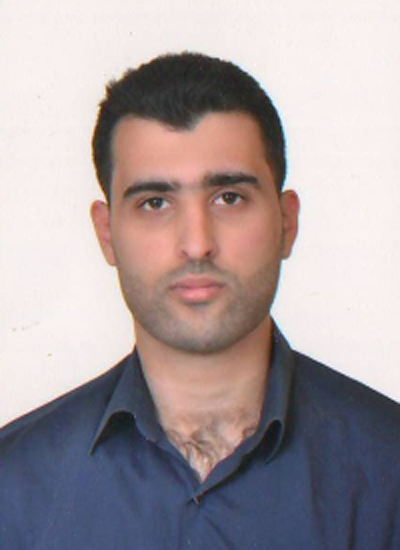
\includegraphics[scale=1]{mypictureCubic.png}
	\end{center}
	\caption{My Picture Cubic} 
\end{figure}
In Cubic we notice that it's less blur than Bilinear and less squares than nearest neighbor.
\begin{figure}[H]
	\begin{center}
		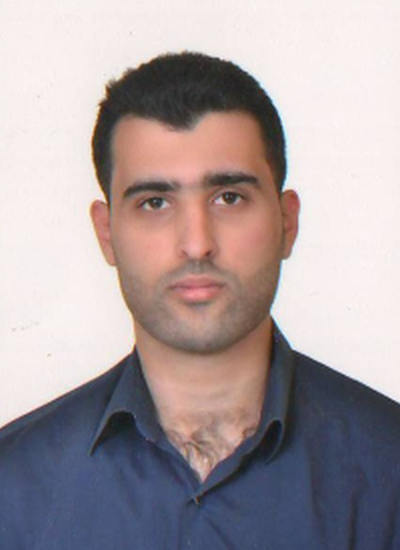
\includegraphics[scale=1]{mypicturespline.png}
	\end{center}
	\caption{My Picture Spline} 
\end{figure}
Even less squares specially near the eyebrows.
\begin{figure}[H]
\begin{center}
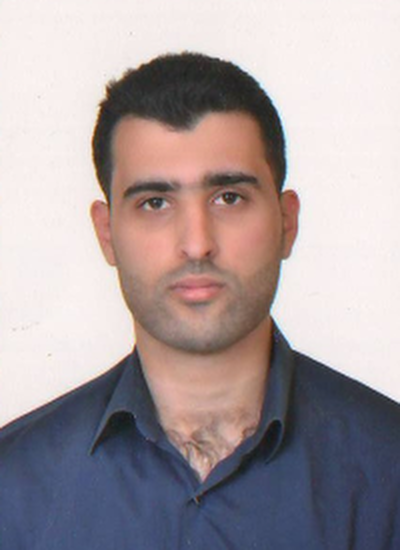
\includegraphics[scale=1]{mypictureLanczos.png}
\end{center}
\caption{Lanczos4 }
\end{figure}
Although lanczos is the most expensive one in time but in this example didn't give the result I expect to be honest. Spline got a better result.
\begin{flushleft}

\end{flushleft}

Since spline was spoused to be a built-in function I used this copied code to calculate it :\cite{10}\\

\begin{lstlisting}[language=matlab]
%THIS CODE IS COPIED FROM THIS REPOSITORY 
%https://www.reddit.com/r/matlab/comments/32vfj0/using_interp2_to_resize_an_imageinstead_of/

cd ('/home/aqeel/Study/IP/hw1/')
%M = imread('mupictureorignalgrayscal.png');
M = imread('Obelexorignalgrayscal.png');
t = cputime;
M = double(M);

[Y,X,z] = size(M);
MaxD = max(size(M));
%Scale = 550/MaxD; % create the scale to be applied to both dimensions
Scale = 466/MaxD;
[x,y] = meshgrid(1:X,1:Y); % the grid for the original image

[Xq,Yq] = meshgrid(1:Scale*X,1:Scale*Y); % the grid for the new image

MqR = interp2(x,y,M(:,:,1),Xq,Yq,'spline');
MqG = interp2(x,y,M(:,:,2),Xq,Yq,'spline');
MqB = interp2(x,y,M(:,:,3),Xq,Yq,'spline');

Mq = zeros(floor(Scale*Y),floor(Scale*X),3); % initialize new image matrix

Mq(:,:,1) = MqR;
Mq(:,:,2) = MqG;
Mq(:,:,3) = MqB;

Mq = uint8(Mq);

Xi = linspace(1,X,round(X)*Scale);
Yi = linspace(1,Y,round(Y)*Scale);

[Xq,Yq] = meshgrid(Xi,Yi); % **why do I have to swap the X and Y places in the argument??**

Mq = zeros(floor(Y*Scale),floor(X*Scale),3);

for i = 1:3
Mq(:,:,i) = interp2(M(:,:,i),Xq,Yq,'spline');
end

Mq = uint8(Mq);
e = cputime-t
imwrite(Mq,'oblexspline.png')
%imwrite(Mq,'mypicturespline.png')
\end{lstlisting} Code Source\cite{10}

\textbf{Note:}All resources for this home work is available at \href{https://github.com/aqeel13932/IP/tree/master/hw1}{ my repository.}
\begin{thebibliography}{9}
	\bibitem{9}
	Wilhelm Burger, Mark J. Burge (2009). Principles of digital image processing: core algorithms. Springer. pp. 231–232. ISBN 978-1-84800-194-7.
	\bibitem{10}
	\href{https://www.reddit.com/r/matlab/comments/32vfj0/using_interp2_to_resize_an_imageinstead_of/}{Code Source for spline}
	

\end{thebibliography}
\end{document}